\documentclass[onecolumn, compsoc,11pt]{IEEEtran}
\usepackage{paralist}
\usepackage{enumitem}
\usepackage{etex}
\usepackage{amssymb,amsfonts,amsmath,amsthm}
\usepackage{graphicx}
\usepackage{booktabs}
\usepackage[usenames,x11names, dvipsnames, svgnames]{xcolor}
\usepackage{amsmath,amssymb}
\usepackage{dsfont}
\usepackage{amsfonts}
\usepackage{mathrsfs}
\usepackage{texshade}
\usepackage{hyperref}
\hypersetup{
  colorlinks=true,
  linkcolor=black,
  citecolor=blue,
  filecolor=black,
  urlcolor=DodgerBlue4,
  breaklinks=false,
  % linkbordercolor=red,% hyperlink borders will be red
  % pdfborderstyle={/S/U/W 1}% border style will be underline of width 1pt
}
\usepackage{array}
\usepackage{xr}
\usepackage{verbatim}
\usepackage{multirow}
\usepackage{longtable}
\usepackage{tikz-network}
\usepackage[T1,euler-digits]{eulervm}
\usepackage{times}
% \usepackage{pxfonts}
\usepackage{tikz}
\usepackage{pgfplots}
\usetikzlibrary{shapes,calc,shadows,fadings,arrows,decorations.pathreplacing,automata,positioning}
\usetikzlibrary{external}
\usetikzlibrary{decorations.text}
\usepgfplotslibrary{colorbrewer} 
\usepgfplotslibrary{statistics}

\tikzexternalize[prefix=./Figures/External/]% activate externalization!
\tikzexternaldisable
% \addtolength{\voffset}{.1in}  
\usepackage{geometry}
\geometry{letterpaper, left=.6in,right=.6in,top=.5in,bottom=0.7in}

%\addtolength{\textwidth}{-.1in}    
%\addtolength{\hoffset}{.05in}    
%\addtolength{\textheight}{.1in}    
%\addtolength{\footskip}{0in}    
\usepackage{rotating}
\definecolor{nodecol}{RGB}{240,240,220}
\definecolor{nodeedge}{RGB}{240,240,225}
\definecolor{edgecol}{RGB}{130,130,130}
\tikzset{%
  fshadow/.style={      preaction={
      fill=black,opacity=.3,
      path fading=circle with fuzzy edge 20 percent,
      transform canvas={xshift=1mm,yshift=-1mm}
    }} 
}
\usetikzlibrary{pgfplots.dateplot}
\usetikzlibrary{patterns}
\usetikzlibrary{decorations.markings}
\usepackage{fancyhdr}
\usepackage{mathtools}
\usepackage{datetime}
\usepackage{comment}
%% ## Equation Space Control---------------------------
\def\EQSP{3pt}
\newcommand{\mltlne}[2][\EQSP]{\begingroup\setlength\abovedisplayskip{#1}\setlength\belowdisplayskip{#1}\begin{equation}\begin{multlined} #2 \end{multlined}\end{equation}\endgroup\noindent}
\newcommand{\cgather}[2][\EQSP]{\begingroup\setlength\abovedisplayskip{#1}\setlength\belowdisplayskip{#1}\begin{gather} #2 \end{gather}\endgroup\noindent}
\newcommand{\cgathers}[2][\EQSP]{\begingroup\setlength\abovedisplayskip{#1}\setlength\belowdisplayskip{#1}\begin{gather*} #2 \end{gather*}\endgroup\noindent}
\newcommand{\calign}[2][\EQSP]{\begingroup\setlength\abovedisplayskip{#1}\setlength\belowdisplayskip{#1}\begin{align} #2 \end{align}\endgroup\noindent}
\newcommand{\caligns}[2][\EQSP]{\begingroup\setlength\abovedisplayskip{#1}\setlength\belowdisplayskip{#1}\begin{align*} #2 \end{align*}\endgroup\noindent}
\newcommand{\mnp}[2]{\begin{minipage}{#1}#2\end{minipage}} 
%% COLOR DEFS------------------------------------------
\newtheorem{thm}{Theorem}
\newtheorem{cor}{Corollary}
\newtheorem{lem}{Lemma}
\newtheorem{prop}{Proposition}
\newtheorem{defn}{Definition}
\newtheorem{exmpl}{Example}
\newtheorem{rem}{Remark}
\newtheorem{notn}{Notation}
%% ------------PROOF INCLUSION -----------------
\def\NOPROOF{Proof omitted.}
\newif\ifproof
\prooffalse % or \draftfalse
\newcommand{\Proof}[1]{
  \ifproof
  \begin{IEEEproof}
    #1\end{IEEEproof}
  \else
  \NOPROOF
  \fi
}
%% ------------ -----------------
\newcommand{\DETAILS}[1]{#1}
%% ------------ -----------------
% color commands------------------------
\newcommand{\etal}{\textit{et} \mspace{3mu} \textit{al.}}
% \renewcommand{\algorithmiccomment}[1]{$/** $ #1 $ **/$}
\newcommand{\vect}[1]{\textbf{\textit{#1}}}
\newcommand{\figfont}{\fontsize{8}{8}\selectfont\strut}
\newcommand{\hlt}{ \bf \sffamily \itshape\color[rgb]{.1,.2,.45}}
\newcommand{\pitilde}{\widetilde{\pi}}
\newcommand{\Pitilde}{\widetilde{\Pi}}
\newcommand{\bvec}{\vartheta}
\newcommand{\algo}{\textrm{\bf\texttt{GenESeSS}}\xspace}
\newcommand{\xalgo}{\textrm{\bf\texttt{xGenESeSS}}\xspace}
\newcommand{\FNTST}{\bf }
\newcommand{\FNTED}{\color{darkgray} \scriptsize $\phantom{.}$}
\renewcommand{\baselinestretch}{.9}
\newcommand{\sync}{\otimes}
\newcommand{\psync}{\hspace{3pt}\overrightarrow{\hspace{-3pt}\sync}}
% \newcommand{\psync}{\raisebox{-4pt}{\begin{tikzpicture}\node[anchor=south] (A) {$\sync$};
%   \draw [->,>=stealth] ([yshift=-2pt, xshift=2pt]A.north west) -- ([yshift=-2pt]A.north east); %\end{tikzpicture}}}
\newcommand{\base}[1]{\llbracket #1 \rrbracket}
\newcommand{\nst}{\textrm{\sffamily\textsc{Numstates}}}
\newcommand{\HA}{\boldsymbol{\mathds{H}}}
\newcommand{\eqp}{ \vartheta }
\newcommand{\entropy}[1]{\boldsymbol{h}\left ( #1 \right )}
\newcommand{\norm}[1]{\left\lVert #1 \right\rVert}%
\newcommand{\abs}[1]{\left\lvert #1 \right\rvert}%
\newcommand{\absB}[1]{\big\lvert #1 \big\rvert}%
% #############################################################
% #############################################################
% PREAMBLE ####################################################
% #############################################################
% #############################################################
% \usepackage{pnastwoF}      
\DeclareMathOperator*{\argmax}{argmax}
\DeclareMathOperator*{\argmin}{arg\,min}
\DeclareMathOperator*{\expect}{\mathbf{E}}
\DeclareMathOperator*{\var}{\mathbf{Var}}

\newcommand{\ND}{ \mathcal{N}  }
\usepackage[linesnumbered,ruled,vlined,noend]{algorithm2e}
\newcommand{\captionN}[1]{\caption{\color{darkgray} \sffamily \fontsize{9}{10}\selectfont #1  }}
\newcommand{\btl}{\ \textbf{\small\sffamily bits/letter}}
%\usepackage{txfonts}
%%% \usepackage{ccfonts}
%%% save defaults
%\renewcommand{\rmdefault}{phv} % Arial
%\renewcommand{\sfdefault}{phv} % Arial
%\edef\keptrmdefault{\rmdefault}
%\edef\keptsfdefault{\sfdefault}
%\edef\keptttdefault{\ttdefault}

% \usepackage{kerkis}
%\usepackage[OT1]{fontenc}
%\usepackage{concmath}
% \usepackage[T1]{eulervm} 
% \usepackage[OT1]{fontenc}
%%% restore defaults
%\edef\rmdefault{\keptrmdefault}
%\edef\sfdefault{\keptsfdefault}
%\edef\ttdefault{\keptttdefault}
\tikzexternalenable
% ##########################################################
\tikzfading[name=fade out,
inner color=transparent!0,
outer color=transparent!100]
% ###################################
\newcommand{\xtitaut}[2]{
  \noindent\mnp{\textwidth}{
    \mnp{\textwidth}{\raggedright\Huge \bf \sffamily #1}

    \vskip 1em

    {\bf \sffamily #2}
  }
  \vskip 2em
}
% ###################################
% ###################################
\tikzset{wiggle/.style={decorate, decoration={random steps, amplitude=10pt}}}
\usetikzlibrary{decorations.pathmorphing}
\pgfdeclaredecoration{Snake}{initial}
{
  \state{initial}[switch if less than=+.625\pgfdecorationsegmentlength to final,
  width=+.3125\pgfdecorationsegmentlength,
  next state=down]{
    \pgfpathmoveto{\pgfqpoint{0pt}{\pgfdecorationsegmentamplitude}}
  }
  \state{down}[switch if less than=+.8125\pgfdecorationsegmentlength to end down,
  width=+.5\pgfdecorationsegmentlength,
  next state=up]{
    \pgfpathcosine{\pgfqpoint{.25\pgfdecorationsegmentlength}{-1\pgfdecorationsegmentamplitude}}
    \pgfpathsine{\pgfqpoint{.25\pgfdecorationsegmentlength}{-1\pgfdecorationsegmentamplitude}}
  }
  \state{up}[switch if less than=+.8125\pgfdecorationsegmentlength to end up,
  width=+.5\pgfdecorationsegmentlength,
  next state=down]{
    \pgfpathcosine{\pgfqpoint{.25\pgfdecorationsegmentlength}{\pgfdecorationsegmentamplitude}}
    \pgfpathsine{\pgfqpoint{.25\pgfdecorationsegmentlength}{\pgfdecorationsegmentamplitude}}
  }
  \state{end down}[width=+.3125\pgfdecorationsegmentlength,
  next state=final]{
    \pgfpathcosine{\pgfqpoint{.15625\pgfdecorationsegmentlength}{-.5\pgfdecorationsegmentamplitude}}
    \pgfpathsine{\pgfqpoint{.15625\pgfdecorationsegmentlength}{-.5\pgfdecorationsegmentamplitude}}
  }
  \state{end up}[width=+.3125\pgfdecorationsegmentlength,
  next state=final]{
    \pgfpathcosine{\pgfqpoint{.15625\pgfdecorationsegmentlength}{.5\pgfdecorationsegmentamplitude}}
    \pgfpathsine{\pgfqpoint{.15625\pgfdecorationsegmentlength}{.5\pgfdecorationsegmentamplitude}}
  }
  \state{final}{\pgfpathlineto{\pgfpointdecoratedpathlast}}
}
% ###################################
% ###################################
\newcolumntype{L}[1]{>{\rule{0pt}{2ex}\raggedright\let\newline\\\arraybackslash\hspace{0pt}}m{#1}}
\newcolumntype{C}[1]{>{\rule{0pt}{2ex}\centering\let\newline\\\arraybackslash\hspace{0pt}}m{#1}}
\newcolumntype{R}[1]{>{\rule{0pt}{2ex}\raggedleft\let\newline\\\arraybackslash\hspace{0pt}}m{#1}}



% ################################################
% ################################################
% ################################################
% ################################################
\def\DISCLOSURE#1{\def\disclosure{#1}}
\DISCLOSURE{\raisebox{15pt}{$\phantom{XxxX}$This sheet contains proprietary information 
    not to be released to third parties except for the explicit purpose of evaluation.}
}
% ####################################
\newcommand{\set}[1]{\left\{ #1 \right\}}
\newcommand{\paren}[1]{\left( #1 \right)}
\newcommand{\bracket}[1]{\left[ #1 \right]}
% \newcommand{\norm}[1]{\left\Vert #1 \right\Vert}
\newcommand{\nrm}[1]{\left\llbracket{#1}\right\rrbracket}
\newcommand{\parenBar}[2]{\paren{#1\,{\left\Vert\,#2\right.}}}
\newcommand{\parenBarl}[2]{\paren{\left.#1\,\right\Vert\,#2}}
\newcommand{\ie}{$i.e.$\xspace}
\newcommand{\addcitation}{\textcolor{black!50!red}{\textbf{ADD CITATION}}}
\newcommand{\subtochange}[1]{{\color{black!50!green}{#1}}}
\newcommand{\tobecompleted}{{\color{black!50!red}TO BE COMPLETED.}}


\newcommand{\pIn}{\mathscr{P}_{\textrm{in}}}
\newcommand{\pOut}{\mathscr{P}_{\textrm{out}}}
\newcommand{\aIn}[1][\Sigma]{#1_{\textrm{in}}}
\newcommand{\aOut}[1][\Sigma]{#1_{\textrm{out}}}
\newcommand{\xin}[1]{#1_{\textrm{in}}}
\newcommand{\xout}[1]{#1_{\textrm{out}}}

\newcommand{\R}{\mathbb{R}} % Set of real numbers
\newcommand{\F}[1][]{\mathcal{F}_{#1}}
\newcommand{\SR}{\mathcal{S}} % Semiring of sets
\newcommand{\RR}{\mathcal{R}} % Ring of sets
\newcommand{\N}{\mathbb{N}} % Set of natural numbers (0 included)


\newcommand{\Pp}[1][n]{\mathscr{P}^+_{#1}}
\renewcommand{\entropy}[1]{\boldsymbol{h}\left ( #1 \right )}



\makeatletter
\pgfdeclarepatternformonly[\hatchdistance,\hatchthickness]{flexible hatch}
{\pgfqpoint{0pt}{0pt}}
{\pgfqpoint{\hatchdistance}{\hatchdistance}}
{\pgfpoint{\hatchdistance-1pt}{\hatchdistance-1pt}}%
{
  \pgfsetcolor{\tikz@pattern@color}
  \pgfsetlinewidth{\hatchthickness}
  \pgfpathmoveto{\pgfqpoint{0pt}{0pt}}
  \pgfpathlineto{\pgfqpoint{\hatchdistance}{\hatchdistance}}
  \pgfusepath{stroke}
}
\makeatother

\pgfdeclarepatternformonly{north east lines wide}%
{\pgfqpoint{-1pt}{-1pt}}%
{\pgfqpoint{10pt}{10pt}}%
{\pgfqpoint{9pt}{9pt}}%
{
  \pgfsetlinewidth{0.7pt}
  \pgfpathmoveto{\pgfqpoint{0pt}{0pt}}
  \pgfpathlineto{\pgfqpoint{9.1pt}{9.1pt}}
  \pgfusepath{stroke}
}

\pgfdeclarepatternformonly{north west lines wide}%
{\pgfqpoint{-1pt}{-1pt}}%
{\pgfqpoint{10pt}{10pt}}%
{\pgfqpoint{9pt}{9pt}}%
{
  \pgfsetlinewidth{0.7pt}
  \pgfpathmoveto{\pgfqpoint{0pt}{9pt}}
  \pgfpathlineto{\pgfqpoint{9.1pt}{-0.1pt}}
  \pgfusepath{stroke}
}
\makeatletter

\pgfdeclarepatternformonly[\hatchdistance,\hatchthickness]{flexible hatchB}
{\pgfqpoint{0pt}{\hatchdistance}}
{\pgfqpoint{\hatchdistance}{0pt}}
{\pgfpoint{1pt}{\hatchdistance-1pt}}%
{
  \pgfsetcolor{\tikz@pattern@color}
  \pgfsetlinewidth{\hatchthickness}
  \pgfpathmoveto{\pgfqpoint{0pt}{\hatchdistance}}
  \pgfpathlineto{\pgfqpoint{\hatchdistance}{0pt}}
  \pgfusepath{stroke}
}    \makeatother


\def\TPR{\textrm{TPR}\xspace}
\def\TNR{\textrm{TNR}\xspace}
\def\FPR{\textrm{FPR}\xspace}
\def\PPV{\textrm{PPV}\xspace}

\usetikzlibrary{arrows.meta}
\usetikzlibrary{decorations.pathreplacing,shapes.misc}
\usepgfplotslibrary{fillbetween}
%usepackage{tikz-network}
\usetikzlibrary{shapes.geometric}
\usetikzlibrary{math}
\usepgfplotslibrary{colorbrewer} 

\usepackage{textcomp}
\usepackage{colortbl}
\usepackage{array}
\usepackage{courier} 
\usepackage{wrapfig}
\usepackage{pifont}
\usetikzlibrary{chains,backgrounds}
\usetikzlibrary{intersections}
\usetikzlibrary{pgfplots.groupplots}
\usepgfplotslibrary{fillbetween} 
\usetikzlibrary{arrows.meta}
\usepackage{pgfplotstable}
\usepackage[super,compress,sort,comma]{natbib}
%\usepackage{natbib}
\usepackage{setspace}
\usetikzlibrary{math}
\usetikzlibrary{matrix}
\usepackage{xstring}
\usepackage{xspace}
\usepackage{flushend}
\makeatletter
\renewcommand\section{\@startsection {section}{1}{\z@}%
  {-2ex \@plus -1ex \@minus -.2ex}%
  {1ex \@plus.1ex}%
  {\Large\bfseries\scshape}}
\renewcommand\subsection{\@startsection {subsection}{1}{\z@}%
  {-2ex \@plus -.25ex \@minus -.2ex}%
  {0.1ex \@plus.0ex}%
  {\fontsize{11}{10}\selectfont\bfseries\sffamily\color{black}}}
\renewcommand\subsubsection{\@startsection {subsubsection}{1}{\z@}%
  {0ex \@plus -.5ex \@minus -.2ex}%
  {0.0ex \@plus.5ex}%
  {\bfseries\itshape\sffamily\color{darkgray}}}
\renewcommand\paragraph{\@startsection {paragraph}{1}{\z@}%
  {-.2ex \@plus -.5ex \@minus -.2ex}%
  {0.0ex \@plus.5ex}%
  {\fontsize{9}{9}\selectfont\itshape\sffamily\color{darkgray}}}
       
%\renewcommand{\thesubsection}{\thesection.\arabic{subsection}}
\renewcommand{\thesubsectiondis}{\arabic{subsection}.}
\renewcommand{\thesectiondis}{\arabic{section}.}
\renewcommand{\thesection}{\arabic{section}}

\renewcommand{\thetable}{\arabic{table}}

\makeatother
\makeatletter
\pgfdeclareradialshading[tikz@ball]{ball}{\pgfqpoint{-10bp}{10bp}}{%
  color(0bp)=(tikz@ball!30!white);
  color(9bp)=(tikz@ball!75!white);
  color(18bp)=(tikz@ball!90!black);
  color(25bp)=(tikz@ball!70!black);
  color(50bp)=(black)}
\makeatother
%\newcommand{\tball}[1][CadetBlue4]{${\color{#1}\Large\boldsymbol{\blacksquare}}$}
\renewcommand{\baselinestretch}{1}
%\renewcommand{\captionN}[1]{\caption{\color{CadetBlue4!50!black} \sffamily \fontsize{9}{10}\selectfont #1  }}
\tikzexternaldisable 
\parskip=6pt
\parindent=0pt
%\newcommand{\Mark}[1]{\textsuperscript{#1}}
\pagestyle{fancy}

\newcounter{Dcounter}
\setcounter{Dcounter}{1}
\newcommand{\DQS}[1]{\marginpar{\tikzexternaldisable \tikz{\node[rounded corners=5pt,draw=none,thick,fill=black!10,font=\sffamily\fontsize{7}{8}\selectfont] {\mnp{.45in} {\color{Red3}\raggedright  \#\theDcounter.~#1}}; }}\stepcounter{Dcounter}\xspace}

\newcommand{\qn}[1][i]{\Phi_{#1}}
\newcommand{\D}[1][i]{\mathscr{D}\left ( {\Sigma_#1} \right ) }
\newcommand{\Dx}{\mathscr{D}}
\def\J{\mathds{J}}
\def\M{\omega}
\def\N{\mathds{N}}
\newcommand{\cp}[1][P]{\langle #1 \rangle}
\newcommand{\mem}[1]{\M_{#1}}


\makeatletter
\newcommand\transformxdimension[1]{
    \pgfmathparse{((#1/\pgfplots@x@veclength)+\pgfplots@data@scale@trafo@SHIFT@x)/10^\pgfplots@data@scale@trafo@EXPONENT@x}
}
\newcommand\transformydimension[1]{
    \pgfmathparse{((#1/\pgfplots@y@veclength)+\pgfplots@data@scale@trafo@SHIFT@y)/10^\pgfplots@data@scale@trafo@EXPONENT@y}
}
\makeatother

\parskip=6pt
\parindent=0pt


\pgfplotsset{
    discard if/.style 2 args={
        x filter/.code={
            \edef\tempa{\thisrow{#1}}
            \edef\tempb{#2}
            \ifx\tempa\tempb
                \def\pgfmathresult{inf}
            \fi
        }
    },
    discard if not/.style 2 args={
        x filter/.code={
            \edef\tempa{\thisrow{#1}}
            \edef\tempb{#2}
            \ifx\tempa\tempb
            \else
                \def\pgfmathresult{inf}
            \fi
        }
    }
  }

  %\newcommand{\HLT}[2][Red1]{{\color{#1}#2}}

 % \def\commatonone{\expandafter\zappointzerozero
%    \romannumeral`\^^@}
%\def\zappointzerozero#1.00{\zapcomma#1,!}
%\def\zapcomma#1,#2{#1\ifx!#2\else#2\expandafter\zapcomma\fi}
\def\commatononei#1,{#1}
\def\commatononej#1,#2,{#1#2}
\def\commatonone#1{\expandafter\commatononei#1}
\def\commatononeT#1{\expandafter\commatononej#1}
\newcommand{\Sum} [2] {#1 + #2 = \the\numexpr #1 + #2 \relax \\}


\usepackage{sistyle}
\SIthousandsep{,}

\makeatletter
\newcommand{\limitpages}[1]{
  \gdef\maxpages{#1}%
  \ifx\latex@outputpage\@undefined\relax%
  \global\let\latex@outputpage\@outputpage%
  \fi%
  \gdef\@outputpage{%
    \ifnum\value{page}>\maxpages\relax%
    % Do not output the page
    \else%
    \latex@outputpage%
    \fi%
  }%
}
\makeatother
\newcommand{\note}[1]{{ \itshape \footnotesize \color{Red1}$\medbullet$~ #1}}









\renewcommand{\thesectiondis}{\arabic{section}.}
\renewcommand{\thesubsectiondis}{\Alph{subsection}.}

\makeatletter
\renewcommand\section{\@startsection {section}{1}{\z@}%
  {-1pt \@plus -30ex \@minus 20ex}%
  {.1pt}%
  {\large\bfseries\scshape}}
\renewcommand\subsection{\@startsection {subsection}{2}{\z@}%
  {0ex \@plus -1.75ex \@minus -1.2ex}%
  {0ex \@plus.0ex}%
  {\fontsize{11}{11}\selectfont\bfseries\sffamily\color{black}}}
\renewcommand\subsubsection{\@startsection {section}{1}{\z@}%
  {-.1ex \@plus -.5ex \@minus -.2ex}%
  {0.0ex \@plus.5ex}%
  {\bfseries\sffamily\color{Red4}}}
\renewcommand\paragraph{\@startsection {section}{1}{\z@}%
  {-.1ex \@plus -.5ex \@minus -.2ex}%
  {0.0ex \@plus.5ex}%
  {\fontsize{11}{10}\selectfont\bfseries\itshape\sffamily\color{black}}}
\makeatother


\makeatletter
\pgfdeclareradialshading[tikz@ball]{ball}{\pgfqpoint{-10bp}{10bp}}{%
  color(0bp)=(tikz@ball!30!white);
  color(9bp)=(tikz@ball!75!white);
  color(18bp)=(tikz@ball!90!black);
  color(25bp)=(tikz@ball!70!black);
  color(50bp)=(black)}
\makeatother
\newcommand{\tball}{${\color{CadetBlue3}\Large\boldsymbol{\blacksquare}}$}
\renewcommand{\baselinestretch}{.87}
\newcommand{\VSP}{\vspace{-2pt}}
\renewcommand{\captionN}[1]{\caption{\color{black} \sffamily \fontsize{9}{10}\selectfont #1  }}




\newcommand*{\doi}[1]{\href{http://dx.doi.org/#1}{doi: #1}}
\renewcommand{\IEEEbibitemsep}{20pt plus 2pt}
\makeatletter
\IEEEtriggercmd{\reset@font\normalfont\fontsize{11}{14}\selectfont}
\makeatother
\IEEEtriggeratref{1}
\newlength{\bibitemsep}\setlength{\bibitemsep}{.2\baselineskip plus .05\baselineskip minus .05\baselineskip}
\newlength{\bibparskip}\setlength{\bibparskip}{0pt}
\let\oldthebibliography\thebibliography
\renewcommand\thebibliography[1]{%
  \oldthebibliography{#1}%
  \setlength{\parskip}{\bibitemsep}%
  \setlength{\itemsep}{\bibparskip}%
}
\setlength{\bibitemsep}{.3\baselineskip plus .05\baselineskip minus .05\baselineskip}
\usepackage{pgfgantt}
\usepackage{textcomp}
\usepackage{colortbl}
\usepackage{subfigure}
\usepackage{array}
\usepackage{courier}
\usepackage{setspace} 
\usepackage{wrapfig} 
\usepackage{calligra}
%\usepackage{ulem}
\usepackage{multirow}



\usetikzlibrary{chains,backgrounds}
\usetikzlibrary{intersections}
\usepackage{xstring}
\usepackage{wasysym}
\usepackage[misc]{ifsym}
\tikzexternaldisable 
\parskip=4pt
\parindent=0pt
\lhead{}
\pagestyle{empty}
\lfoot{}
\pagestyle{fancy}
\def\COLA{black}
% ###################################
\cfoot{\bf\sffamily \scriptsize \color{Maroon!50} I. Chattopadhyay, Department of Medicine, University of Chicago}
\cfoot{}
\rhead{}
\newcommand{\partxt}{\bf\sffamily\itshape}
% ############################################################
\newif\iftikzX
\tikzXtrue
\tikzXfalse

% ############################################################
\addtolength{\voffset}{.1in}
\addtolength{\textwidth}{-.085in}
\addtolength{\hoffset}{.0425in}
\def\PROG{Mallinckrodt\xspace}
\def\ZERO{ACoR\xspace}
\def\COLWA{\XCOLA!40}
\def\COLWB{\XCOLD!20}
\def\COLWC{\XCOLA!40}
\def\COLWD{\XCOLD!20}
\def\COLWE{\XCOLA!40}
\def\COLWF{\XCOLD!20}
\def\infl{Influenza A\xspace}
\def\enet{Emergenet\xspace}
% ############################################################
\def\treatment{positive\xspace}
\def\SUPPLEMENTARY{Supplementary\xspace}
\def\METHODS{Online Methods\xspace}
\def\EXTENDED{Extended Data\xspace}
\def\TITLE{BioNORAD:  Scalable Emergence Risk Assessment of Animal \infl}

\begin{document} 

\lhead{\textbf{\TITLE}}

\limitpages{5}
%\HDR

%\section*{Project Narrative}
% – Rationale: Clearly articulate the scientific rationale for the proposed research
% project. Cite relevant literature. The presentation of preliminary and/or published
% data is allowed but not required.
\def\bnd{BioNORAD\xspace}
\subsubsection*{Rationale}
% \begin{wrapfigure}[24]{r}{2.5in}
%   \hspace{-15pt}\includegraphics[width=2.65in]{Figures/External/f01}

%   \vspace{-10pt}
  
%   \hspace{-5pt}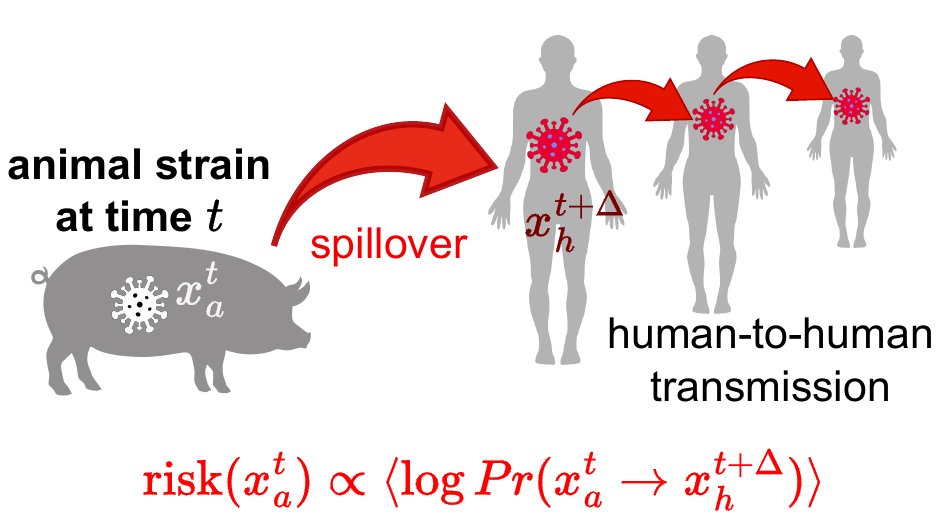
\includegraphics[width=2.5in]{Figures/External/f02}
%   \vspace{-12pt} 
  
%   \captionN{Theoretical foundation of \bnd}\label{fig0}
% \end{wrapfigure}
\infl, partly on account of its segmented genome and its wide prevalence in animal hosts, has the ability to incorporate genes from multiple strains and (re)emerge as novel human pathogens~\cite{reid2003origin,dos2016influenza}, thus harboring  a high pandemic potential. Strains spilling over into humans from animal reservoirs is thought to have triggered  mild to devastating pandemics  at least 4 times (1918 Spanish flu/H1N1, 1957 Asian flu/H2N2, 1968 Hong Kong flu/H3N2, 2009 swine flu/H1N1) in the past century~\cite{shao2017evolution}. One  approach to mitigating such risk is to recognize  animal strains  that do not yet circulate in humans, but are likely to spill-over and quickly achieve human-to-human (HH) transmission capability. While global surveillance efforts collect  wild specimens from diverse hosts/locations annually, our  ability to reliably and scalably  risk-rank individual strains remains limited~\cite{wille2021accurately}. CDC's current solution to this problem is the Influenza Risk Assessment Tool (IRAT)~\cite{Influenz24:online}.  Strain scoress based multiple experimentakl assays,  the number of  human infections if any, transmission in laboratory animals, receptor binding, population immunity, genomic analysis, antigenic relatedness, global prevalence,  pathogenesis, and  treatment options,  are averaged to estimate emergence IRAT score, a number between 1 and 10.  IRAT scores  take  weeks/months to compile for a single strain. With tens of   thousands of strains being collected annually, this results in  a scalability bottleneck.


Here we plan to develop a platform powered by  pattern discovery and a novel generative AI framework to analyze all \infl strains currently in public repositories,  to  parse  emergent evolutionary constraints operating  in the wild. We plan to show   that this capability enables preempting  strains which are \textit{expected to be in future human circulation}, and  approximate IRAT scores of non-human strains without  experimental assays or SME scoring, in seconds as opposed to weeks or months. Our approach automatically takes into account the time-sensitive variations in selection pressures as the background strain circulation evolves, and will potentially be able to rank-order strains adaptively.

Additionally, we plan to validate our ability to predict future variations of viral proteins by showing that predicted variants of HA are functional, and maintain replicative fitness in cell cultures, and animal models.   Bringing together rigorous data-driven modeling, and validation via tools from reverse genetics we plan to deliver an actionable and deployable platform (the \bnd) that optimally exploits the current biosurvellance capacity,  \textit{identifying when and where an imminent  emergence event is likely, and if any specific animal strain is close to achieving human adaptability and  human-to-human transmission capability.}

Our broader goal in this work is to develop a general framework for foundational discovery in  pathogen zoonosis,  beyond the primary focus  of understanding \infl emergence.

  \subsubsection*{Specific Aims}

\textbf{Aim 1: Develop a predictive framework for viral evolution and emergence risk assessment. (Lead: I. Chattopadhyay (UK))}  
We aim to quantify the probability of spontaneous viral mutation and cross-species transmission. By analyzing large-scale influenza genome datasets, the proposed Emergenet will infer cross-mutation dependencies and evolutionary constraints, enabling real-time forecasting of high-risk strains. The goal is to replace subjective expert-driven assessments with a probabilistic model capable of ranking strains by emergence potential, and identify a small actionable set of strains at teh edge of emergence.

\textbf{Aim 2: Experimentally validate the predictive accuracy of Emergenet. (Lead: S. Chattopadhyay (UK) and Manicassamy (UIowa)) }  
This aim involves generating viral variants predicted by Emergenet through reverse genetics and assessing their fitness in human lung epithelial cells. The replication efficiency, antigenic properties, and transmission potential of these strains will be tested to determine if Emergenet's forecasts align with biological viability. Competitive fitness assays will evaluate whether mutations predicted by Emergenet enhance viral survival, distinguishing them from randomly introduced mutations that result in loss of function.

\textbf{Aim 3: Deploy BioNORAD for real-time pandemic risk surveillance. (Lead: I. Chattopadhyay (UK))}  
This aim integrates Emergenet’s predictive capabilities into an automated global biosurveillance platform. BioNORAD will continuously score and rank emerging influenza strains in real-time using surveillance data from NCBI and GISAID. The system will dynamically update risk profiles, offering public health agencies an early warning system for emerging threats. By comparing BioNORAD's predictive rankings with actual outbreak data, the project will assess its ability to preemptively identify pandemic-potential strains.



\begin{figure}[t]
  
 \mnp{.65\textwidth}{ 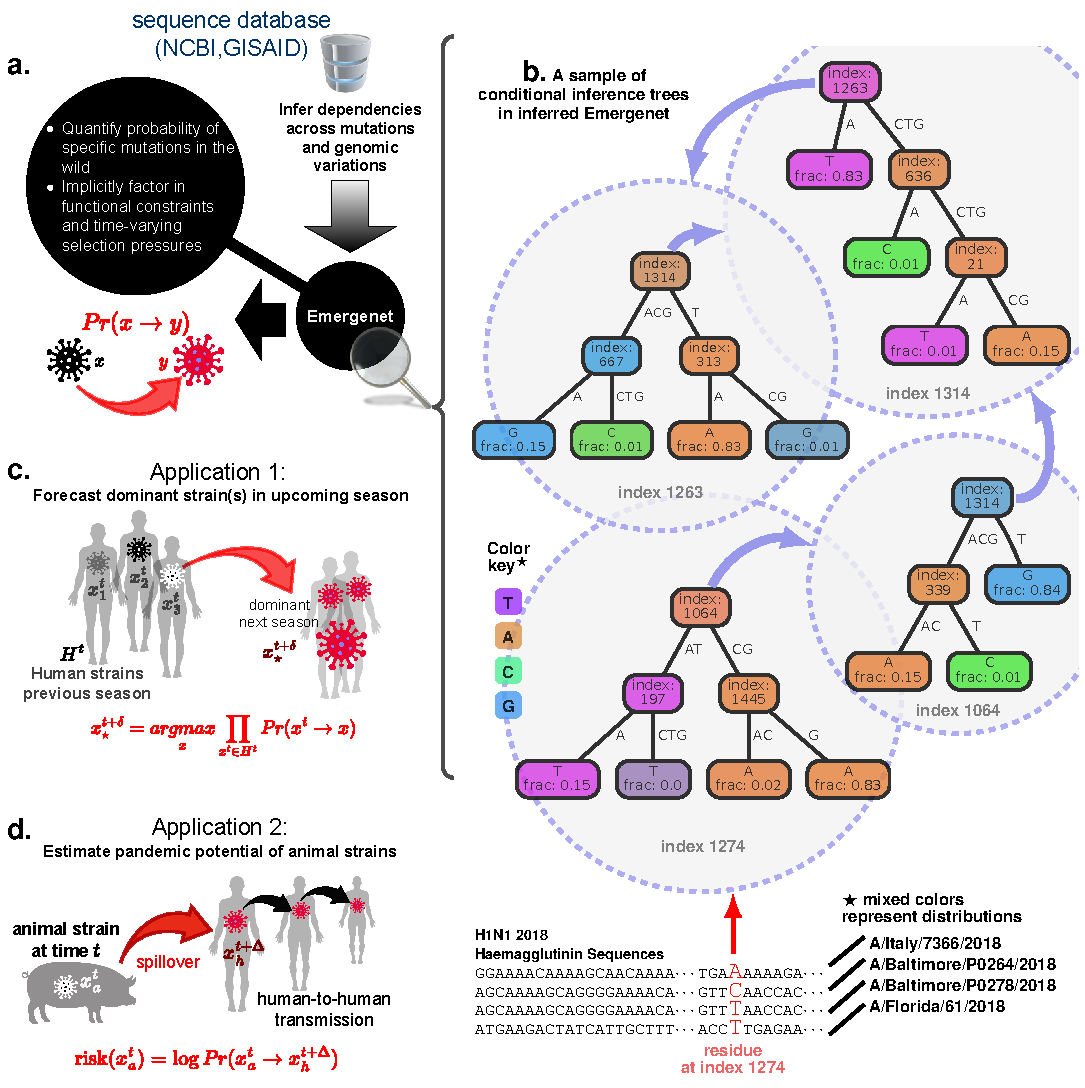
\includegraphics[width=\textwidth]{../overleaf/Figures/External/scheme}
}\hspace{15pt}\mnp{.28\textwidth}{ \captionN{\textbf{Conceptual Scheme: \enet inference}. \textbf{Panel a} Variations of genomes for identical subtypes of \infl are analyzed to infer a recursive forest of conditional inference trees~\cite{Hothorn06unbiasedrecursive} -- the \enet --   which maximally captures the emergent  dependencies between an a priori unspecified number of   mutations. With these inferred dependencies we aim to   estimate the numerical odds of specific mutations, and by extension, the numerical value of the probability of one strain giving rise to another in the wild, under  complex selection pressures from the background. \textbf{Panel b} Snapshot of decision trees  from the \enet inferred for H1N1 HA sequences collected in 2020-2021, which reveals a cyclic dependency~\cite{wu2024emergenet}. In general, every internal node of a component tree can be ``expanded'' into its own tree, underscoring the recursive structure of the \enet. \textbf{Panel c} First application: forecast  dominant strain(s) for the next flu season, using only  sequences collected up to six months prior and the inferred \enet, using data from the past year. \textbf{Panel d} Second application: estimation of the pandemic risk posed by individual animal strains that are still not known to circulate in humans.}\label{fig1}}

  \vspace{-20pt}

  
\end{figure}

\textbf{Aim 2 objectives do not constitute gain-of-function research.} The introduced mutations are  limited to those observed in naturally circulating strains, ensuring no artificial enhancement of transmissibility or pathogenicity. All experimental work will comply with stringent biosafety regulations under BSL-2/BSL-3 conditions, with oversight from institutional biosafety committees. The primary objective is to validate Emergenet’s ability to predict naturally occurring mutations, not to engineer novel viral properties. The focus is on understanding evolutionary trajectories rather than enhancing viral capabilities, aligning fully with ethical and biosafety standards.

\subsubsection*{Foundational Questions Investigated} What drives a viral strain to become pandemic after spill-over events, which tend to be common? Can these events be characterized and preempted? Is sequence-level information sufficient for such predictions? Do historical sequence variations reveal discernible patterns that enable forecasting of future mutations within current circulating populations?

\subsubsection*{Feasibility \& Preliminary Results}
The Emergenet framework has already demonstrated its predictive capability in forecasting the evolutionary trajectories of influenza A strains. By constructing a digital twin of sequence evolution, Emergenet quantitatively assesses the emergence potential of animal strains, providing a scalable alternative to labor-intensive expert assessments. Using a dataset of 220,151 hemagglutinin (HA) sequences, Emergenet outperforms WHO’s seasonal vaccine recommendations for H1N1 and H3N2 subtypes over a 20-year period, improving antigenic match predictions by an average of 3.73 amino acids (28.40\%). Furthermore, Emergenet’s generative models correlate strongly with CDC’s expert-assessed Influenza Risk Assessment Tool (IRAT) scores (Pearson’s r = 0.721, p = $10^{-4}$) while achieving a computational speedup of at least five orders of magnitude, reducing assessment time from months to seconds~\cite{wu2024emergenet}.

\lhead{}

To experimentally validate Emergenet, high-risk HA variants will be generated using the reverse genetics system developed by the BM at U of Iowa. HA segments with predicted mutations will be synthesized and assessed for cell surface expression via flow cytometry and western blotting. Recombinant viruses carrying mutant HA will be generated and validated using next-generation sequencing (NGS). Replication fitness of these recombinant viruses will be evaluated through single-cycle and multicycle replication assays in human lung epithelial cells (A549) and primary human lung cells. Additionally, competition assays between predicted high-fitness mutants and parental strains will be performed in a 1:1 ratio, with fitness outcomes determined via high-resolution melting (HRM) analysis. These experiments will assess the biological relevance of Emergenet’s forecasts, determining whether the predicted mutations enhance viral fitness in human-relevant models.

To further extend the validation framework, SC at UK will conduct in vivo assessments using a well-characterized animal models to determine the pathogenicity and transmissibility of high-risk recombinant influenza variants. Disease severity will be evaluated through body weight loss, lung viral titers, histopathological analysis, and cytokine profiling, and transmission studies will assess whether predicted high-risk strains demonstrate increased transmissibility compared to parental strains in cohoused naive animals. These studies will provide physiological and immunological validation of Emergenet’s predictions, ensuring that computationally inferred high-risk variants correspond to enhanced virulence and transmissibility in a mammalian host.

% The chosen experimental models—**in vitro replication fitness assays and in vivo mouse pathogenesis studies**—offer a rigorous, multi-tiered validation strategy to assess Emergenet’s predictive accuracy. The combination of **computational modeling, cell-based experiments, and animal studies** ensures that identified high-risk strains are not only theoretically emergent but also functionally viable. Dr. Manicassamy, with over 15 years of experience in human and zoonotic influenza viruses under enhanced BSL2/BSL3 conditions, and Dr. Chattopadhyay, with extensive expertise in influenza pathogenesis in animal models, will oversee experimental validation, ensuring biosafety compliance and robust assessment. This integrated validation framework will establish Emergenet as a powerful tool for pandemic risk assessment, enabling early intervention through targeted surveillance and mitigation strategies.


 \clearpage

%\bibliographystyle{plainnat}
%\bibliography{asdgenenew}
\bibliographystyle{naturemag}
\bibliography{allbib}


\end{document}

